\documentclass[12pt]{report}

\usepackage{amssymb}
\usepackage{amsmath}
\usepackage{amsthm}
\usepackage{tikz}
\usepackage{wrapfig}
\usepackage{amsmath}
\usepackage{mathabx}
\usepackage{tkz-berge}

\newtheorem{theorem}{Theorem}[section]
\newtheorem{lemma}[theorem]{Lemma}
\newtheorem{corallary}[theorem]{Corallary}
\newtheorem{definition}{Definition}

\usetikzlibrary{arrows,chains,matrix,positioning,scopes}

\DeclareMathOperator{\lcm}{lcm}
\DeclareMathOperator{\im}{im}

\title{Group Theory}
\author{Jacob Denson}
\date{\today}

\begin{document}

\maketitle

\chapter{What is a group?}

In 1761, Leonard Euler proved the following theorem. Take the totient function, a mapping that takes a positive integer, and returns the total number of integers less than the integer which are relative prime to that integer. A few examples are shown below.
%
\[ \varphi(1) = 0 \]
%
\[ \varphi(10) = 3 \]
%
Euler showed that, for any two relatively prime integers $a$ and $b$, it always follows that
%
\[ a^{\varphi(b)} \equiv 1 \mod{b} \]
%
Euler's proof involved mapping the set of numbers relatively prime to $b$ to integer multiples of $a$ and showing that, modulo $b$, these sets are the same. Since the ancient Greeks, mathematicians have been attempting to find integer solutions to Diophantine equations, integer values that result in zeroes to polynomial functions. In recent years this have given rise to the study of elliptic curves, an equation in the real plane of the form
%
\[ y^2 = x^3 + Ax + B \]
%
Solutions to these equations interact in interesting ways which mean that the field is still going strong today. The most famous proof in recent history, Fermat's last theorem by Andrew Wiles, showed that these curves have correspondences to modular functions: shapes in the complex plane that have an inherent symmetrical property. Felix Klein in the 19th century attempted to answer questions about geometry by considering the inherent geometric properties of shapes. Everiste Galois had already used these techniques, but to explore the inherent symmetries in algebraic equations and determine the insolvability of the quintic equation. Though from separate fields, all of these problems are addressed by relating the objects to one another through different operations - whether they are symmetries or addition and multiplication of numbers. Though it was not known at the time of these discoveries, we know today the reason why these problems are connected is the objects studied follow the abstract concept of a group. This book attempts to introduce the reader to the concept of a group in order to explain the phenomena expressed above, as well as to show the reader the beauty of the abstract concepts developed.

\chapter{Operations and Groups}

Groups are a way to generalize the notion of a set with a well behaved operation which creates a mechanism to combine objects in that set to form another. Operations on numbers are inherent, as are geometric symmetries. Since groups were defined in 1882 by Walter Dyck, the theory has arisen to become one of the largest fields in modern mathematics: abstract algera. The power obtained from the simple definition of a group is that any proof about an abstract group instantly applies to the large number of concrete objects that fit the mold of a group's definition. The longstanding questions shown above all lead to the group's definition. One of the tricks in every Mathematician's device is to solve a problem, and then to attempt to generalize the method used to solve the problem to apply to other techniques. It is only natural then that Group theory was to be generalized by these problems. It has proved to be one of the most useful ones to be created in the past two centuries.

Groups are intimately connected to the operations that define them. Thus, before we define a group, we must rigorously define what an operation is. Operations are mathematical structures that we use almost everyday -- for example, addition and multiplication of numbers. Thus, it is not surprising that generalizing the properties of everyday operations is quite difficult to see. The formal definition is simple.

\begin{definition}
    A {\bf law of composition} or {\bf assignment} on a set $S$ is a function from $S \times S$ to $S$.
\end{definition}

Think of an operation as a way of combining two elements of $S$ into a new element $S$. Note that in our definition we have inherently incorporated the property of {\bf closure} -- that the composition of any two objects in the set $S$ lies inside the set $S$. If $a$ and $b$ are arguments to this function, the value mapped from $a$ and $b$ is most commonly denoted as $ab$, but also as $a \circ b$, or $a + b$, rather than $f(a,b)$, or some other common symbol commonly used for a function. This makes the notation less chunky, and keeps the intuitive definition of an operation as combinations of elements in our head while we work. A good notation like this can make working with the ideas of groups much simpler. While these symbols above are the most common for groups, any other symbol may be used for the operation. 

We introduce a useful bit of notation to write down associative operations. Consider a finite sequence of elements
%
\[ (x_1,x_2, \dots, x_n) \]
%
Then another notation convenience arises, the aptly named `Pi' notation.
%
\[ \prod_{j = i}^n x_j = \big( \prod_{j = 1}^{n-1} x_j \big) x_i \]
\[ \prod_{j = i}^i x_j = x_j \]
%
Make sure to note the similarity to the $\Sigma$ notation used in sums of numbers.

Calculus is studied by narrowing down the functions it studies to narrower subsets with specific properties, the continuous and differentiable functions. The set of all functions is too general to be studied in totality. This is the same about studying human beings. We have vast differences, so very little can be said about the human race about the whole, but quite a lot can be said about certain groups of humans. As in these cases, the assignment property is too general for our study of groups, and thus we must specify subclasses of assignments which we will begin to study. The following characterizes how a group operates on the set. We will also show properties that elements of the set identify with the assignment.

\begin{definition}
    An assignment on a set is {\bf associative} if for any three elements $a$, $b$, and $c$ in that set, $a(bc) = (ab)c$.
\end{definition}

Altogether, this means any number of brackets written in an equation are irrelevant. The order in which elements are put together, however, is still important! In order to say this however, we must rigorously prove this. A formal specification of this conjecture is the following.

\begin{theorem}[Bracket Equivalence]
Given an associative operation on a set, and a finite sequence $(x_1, x_2, \dots, x_n)$ of elements in that set a sequence of elements in that set, for any positive integers $l$ and $m$ such that $l + m = n$,
\[ \big( \prod_{k=1}^l x_k \big) \big( \prod_{k=1}^m x_{l + k} \big) = \prod_{k=1}^n x_k \]
\end{theorem}
\begin{proof}
    We prove by induction on the number of elements in the sequence $(x_1, \dots, x_n)$. When we have only one element in our sequence, the statement is vacously true; there are no positive integers $l$ and $m$ such that $l + m = 1$. When we have two elements $x_1$ and $x_2$, it of course follows that $l = 1$, $m = 1$, and
    %
    \[ \big( \prod_{k=1}^1 x_k \big) \big( \prod_{k=1}^1 x_{k+1} \big) = x_1 x_2 = \prod_{k=1}^2 x_k \]
    %
    Now suppose for our inductive argument that for any sequence of $n-1$ elements, the statement to be proved holds, where $n-1 \geq 2$. Consider a sequence of $n$ elements $(x_1, x_2, \dots, x_n)$ and two positive numbers $l$ and $m$ such that $l + m = n$. The following calculation below proves the statement needed, where $m \geq 2$, as we need to be able to extract an element from the secon product. The case where $m = 1$ is similar (just remove the product that ranges from 1 to $n-1$ in the equation).

    \begin{align}
        \big( \prod_{k=1}^l x_k \big) \big( \prod_{k=1}^m x_{l + k} \big) &= \big( \prod_{k=1}^l x_k \big) \big( \big( \prod_{k=1}^{m-1} x_{l + k} \big)\ x_m \big)\\
        &= \big( \prod_{k=1}^l x_k \prod_{k=1}^{m-1} x_{l + k} \big)\ x_m\\
        &= \big( \prod_{k=1}^{n-1} x_k \big)\ x_m\\
        &= \prod_{k=1}^n x_k
    \end{align}

    Here (2.1) follows by definition of Pi notation, (2.2) follows from the associativity law, (2.3) results from the inductive hypothesis, and (2.4) follows by definition. Thus by induction our conjecture in proven.
\end{proof}

From now on, whenever an associative operation is used, brackets will not be used in the equation under the understanding that any insertation of brackets results in the same outcome. We will substitute brackets to emphasize parts of an equation, but this is only to aid the reader, and not for any reasons of rigour.

We introduce some notation to ensure the elegance and conciseness of our writing. Given a positive integer $n$, we can describe the exponential of the assignment in the following way:
%
\[ a^n = \underbrace{aa \dots aa}_\text{n times} \]
%
One can easily create a recursive definition to be more rigorous, defined by
%
\[ a^1 = a \]
\[ a^n = (a^{n-1}a) \]
%
Two useful lemmas, though obvious, will be used inherently in the proofs that follow later on in the book.

\begin{lemma} For any two integers $n$ and $m$, and any element $a$ in an associative assignment,
\[ a^{n+m} = a^n a^m \]
\end{lemma}
\begin{proof}
    Let $n$ be arbitrary. We prove by induction on $m$. For $m = 1$,
    %
    \[ a^{n + 1} = a^n a = a^n a^1 \]
    %
    This follows directly from the definition. Now suppose this is true for $m = r - 1$. We will show it must hold for $m = r$.

    \[ a^{n + r} = a^{n + r - 1} a = (a^n a^{r-1}) a = a^n a^r \]
\end{proof}

\begin{lemma}
    For any two integers $n$ and $m$, and for any element $a$,
    \[ (a^n)^m = a^{nm} \]
\end{lemma}
\begin{proof}
    As in the last proof, we use induction on $m$ for a fixed $n$. For $m = 1$,
    \[ (a^n)^1 = a^n = a^{n \cdotp 1} \]
    %
    And by supposing that the lemma holds for $m = r-1$
    \[ (a^n)^r = (a^n)^{r-1} a^n = \underbrace{\ a^{n(r-1)} a^n = a^{n(r-1) + n}\ }_\text{Following from Lemma 2.0.2} = a^{nr} \]
\end{proof}

\begin{definition} Another property of an assignment on a set is {\bf commutivity}: that for any elements $a$ and $b$ in the set, $ab = ba$.
\end{definition}

The power of commutativity is that, given an associative and commmutative operation, we can permute any elements in an equation. Rigorously, we are talking about the following theorem.

\begin{theorem}[Commutative Permutation Equivalence]
    For any finite sequence of elements $(x_1, x_2, \dots, x_n)$ from a set upon which an assignment is defined, and for any permutation $\pi$ on the numbers $1$ to $n$,
    %
    \[ \prod_{k=1}^n x_k = \prod_{k=1}^n x_{\pi(k)} \]
\end{theorem}
\begin{proof}
    We again prove by induction on the number of elements in the sequence. When the number of elements in one, the statement is obvious; the only permutation of one element is the identity permutation. Now suppose for induction that this is true for any permutation of $n-1$ elements. Let $(x_1, \dots, x_n)$ be a sequence of elements, and $\pi$ a permutation of $1$ to $n$. Let $m$ be the number such that $\pi(n) = m$. The following calculation shows we can move $x_m$ to the end of the product.
    %
    \begin{align}
    \prod_{k=1}^n x_k &= \big( \prod_{k=1}^{m-1} x_k \big) \big( x_m \prod_{k=m+1}^n x_k \big)\\
    &= \Big( \big( \prod_{k=1}^{m-1} x_k \big) \big( \prod_{k=m+1}^n x_k \big) \Big)\ x_m
    \end{align}
    %
    We transition from (1.5) to (1.6) by use of both the associativity and commutativity property of the assignment. Now define a new permutation $\varphi$ on the numbers from 1 to n by
    %
    \[ \varphi(x) = \begin{cases} x   & x \leq m - 1\\
                               x-1 & x \geq m + 1\\
                               n   & x = m \end{cases} \]
    %
    What follows is that
    %
    \[ \big( \prod_{k=1}^{m-1} x_k \prod_{k=m+1}^n x_k \big)\ x_m = \big( \prod_{k=1}^{n-1} x_{\varphi(k)} \big)\ x_{m} \]
    %
    As $\varphi$ and $\pi$ are permutations, so is $\pi \circ \varphi^{-1}$. Now if we restrict $\pi \circ \varphi^{-1}$ to only the elements 1 to $n-1$, we still have a permutation, because $n$ is fixed in the permutation.
    %
    \[(\pi \circ \varphi^{-1})(n) = \pi(\varphi^{-1}(n)) = \pi(m) = n \]
    %
    By induction and the fact that $(\pi \circ \varphi^{-1})(n) = m$, it follows that
    %
    \begin{align}
        \big( \prod_{k=1}^{n-1} x_{\varphi(k)} \big)\ x_m &= \big( \prod_{k=1}^{n-1} x_{(\pi \circ \varphi^{-1} \circ \varphi)(k)} \big)\ x_{\pi(n)}\\
        &= \big( \prod_{k=1}^{n-1} x_{\pi(k)} \big)\ x_{\pi(n)}\\
        &= \prod_{k=1}^n x_{\pi(k)}
    \end{align}

    We have shown that arbitrary permutations of elements are equal.
\end{proof}

Commutivity does not always hold in all assignments we work with in this book. It is only if $+$ is used as an operation symbol, it is assumed the operation is commutative. All other assignments will not have this property unless specifically stated.

A subtle property of addition and multiplication has not yet been mentioned. With addition, there is a number 0 such that, for any number $x$,
%
\[x + 0 = 0 + x = 0\]
%
Multiplication has a similar number, the number 1. Both numbers are idempotent; that is, when we combine this number with any other number, the composition of the numbers stays the same. We can generalize this concept to arbitrary elements in the following way.

\begin{definition}
    An {\bf identity} of a set with an assignment is an element that is idempotent with all other elements in the group. We commonly call this element $e$, and its properties can be written by the statement that $ae = ea = a$ for all elements $a$.
\end{definition}

\begin{lemma} If an assignment has an identity, it is unique \end{lemma}
\begin{proof}
    Suppose an assignment has two identites, denoted $e$ and $e'$. Then $ee' = e$ by definition of the identity on $e$, but also $ee' = e'$ by the definition of identity on $e'$. By transitivity of equality, $e = e'$.
\end{proof}

If $\cdotp$ is used as the operation's symbol, we may write $e$ as $1$, and if $+$ is used, we may write the identity as $0$, even though the element is not always a number -- the symbol 1 and 0 just becomes a metaphor to help us think about the identity with more abstract operations.

If a set has an identity, we define, for any element $a$, $a^0 = e$, extending the definition of the exponential. The properties previously proved still hold. this is because $0$ is idempotent in addition,
%
\[a^0 a^n = e a^n = a^n = a^{n+0}\]
%
And zeroes out multiplication,
%
\begin{align*} (a^0)^n &= e^n = e = a^0 = a^{0n} & (a^n)^0 &= e = a^0 = a^{0n} \end{align*}

Another subtle quality of addition and multiplication involves the interconnection between elements of the set. Given a number $a$, there is a number $b$ such that $a + b = 0$. We typically use the symbol $-a$ for $b$, and write the operation more concisely as $a - a$. With multiplication, every non-zero element $a$ has an number $b$ such that $a \cdotp b = 1$. We denote $b$ as $a^{-1}$ or $1/a$, and write the operation as $a/a$. Let us extend this notion to an arbitrary operation.

\begin{definition}
    Given a set with an identity $e$, we say an element $a$ is {\bf invertible} if there is another element $b$ such that $ab = ba = e$. b is normally denoted $a^{-1}$ and called the {\bf inverse} of $a$.
\end{definition}

If $+$ is used for the operation, $-a$ is used for the inverse of the element $a$, and if $\cdotp$ is used, $1/a$ might be used. This continues the metaphor established for identity elements.

Here are some properties common to all inverses. We assume associativity, but not commutivity in the operation used.

\begin{lemma}[Length Inverse Equivalency Lemma] Let $l$ and $r$ and $a$ be arbitrary elements of a set. If $la = e$ and $ar = e$, then $l = r$, and $a$ is invertible \end{lemma}
\begin{proof} For then it follows that $l = le = lar = er = r$. \end{proof}

\begin{lemma}[Uniqueness of inverses] $a^{-1}$ is unique \end{lemma}
\begin{proof} The above property shows any two inverses are the same, for if $x$ and $y$ are two inverses, substitute $x$ for $l$ and $y$ for $r$ in Lemma (1.1.3). \end{proof}

We now understand operations enough to describe the class of objects we will study for the rest of the book, a group.

\begin{definition}
    A {\bf group} is a set with an associative operation that contains a unit element (such that the group is non-empty), and such that every element has an inverse. We say the group is abelian if its operation is commutative as well as associative.
\end{definition}

\begin{definition}
    The {\bf order} of a group is the cardinality of the set that the operation operates on.
\end{definition}

If $n < 0$, define $a^n = (a^{-1})^{n}$. Again, the properties proved hold, but we can now extend exponentiation to any integer. Some easy properties result fairly easily from the definition. They all follow from the fact that the inverse of every element is unique. Let $a$ and $b$ be arbitrary elements of a group:

\begin{lemma} The inverse of an inverse of an element $a$ is $a$. That is, $(a^{-1})^{-1} = a$. \end{lemma}
\begin{proof}
    The proof follows as $a a^{-1} = a^{-1} a = e$ and (2.0.7).
\end{proof}

\begin{lemma} $(ab)^{-1} = b^{-1}a^{-1}$. \end{lemma}
\begin{proof} $(ab)(b^{-1}a^{-1}) = aa^{-1} = e$. \end{proof}

\begin{lemma} Every equation $ax = b$ has a unique solution $x$. \end{lemma}
\begin{proof} $x = ba^{-1}$ is a trivial solution, and is the only solution, as if $x'$ is any other solution such that $ax = ax'$, then $a^{-1}ax = a^{-1}ax'$, which when evaluated gives us $x = x'$.
\end{proof}

We require inverses for a group, but we can weaken this claim only requiring left inverses, that is, for an element $a$, an element $b$ where it is true $ba = e$, but it is not necessarily true that $ab = e$.

\begin{theorem}
    Any set with an associative operation and an identity such that every element has a left inverse contains arbitrary inverses for an elemenent, such that the set is a group.
\end{theorem}
\begin{proof}
    Let $G$ be a set with the properties above, and suppose $a$ is an arbitrary element of $G$. Then there is $b \in G$ such that $ba = e$. $b$ also has a left inverse $c$ such that $cb = e$. But then $b$ has both a left and right inverse, so $a = c$ from Lemma $1.1.3$. But that also means $a$ has a right inverse when substituted for $c$, so $b$ is the inverse of $a$, and since $a$ was arbitrary, all elements are invertible and thus $G$ is a group.
\end{proof}

There are also many examples of groups. We list some interesting ones below. Note you do not need to understand all of these examples until they are mentioned later on in the book. You can just use this page as a reference for the groups we mention. Right now just have a look at a choice few to get a feeling for groups:
\begin{itemize}
    \item The set of integers, rational, real, and complex numbers under addition form the groups $\mathbf{Z}^+$, $\mathbf{Q}^+$, $\mathbf{R}^+$, and $\mathbf{C}^+$.
    \item The same sets with zero removed under the operation of multiplication form the groups $\mathbf{Z}^\times$, $\mathbf{Q}^\times$, $\mathbf{R}^\times$, and $\mathbf{C}^\times$.
    \item The set of bijective functions on a set $X$ under composition form the symmetric group $S_{|X|}$. Note that the order of $S_{|X|}$ is $|X|!$ as this is precisely the number of bijective functions on the set.
    \item For a vector space V, the set of automorphisms under compositions form the general linear group $GL(V)$. An equivalent definition, if the vector space is dimension $n$ in a field $\mathbf{F}$, is the set of invertible $n$ by $n$ matrices with entries in $\mathbf{F}$, which we denote $GL_n(\mathbf{F})$.
    \item Let $S$ be a set, and $G$ a group with operation $\cdotp$. Then the set of functions from $S$ to $G$ form a group with operations $\circ$ defined by $(f \circ g)(x) = f(x) \cdotp g(x)$. If $f$ is in the group, $f^{-1}$ is the set defined by $f^{-1}(x) = f(x)^{-1}$
    \item Consider an $n$-sided regular polyhedron (where regular means each side is equal). Each symmetry on the polyhedron, can be considered a rotational symmmetry or a reflection symmetry. We have $n$ of each kinds of these symmetries, so the group formed by taking compositions of symmetries to form more symmetries forms the Dihedral group $D_n$ of order $2n$. Dihedral groups were what Felix Klein was studying in transformational geometry.
    \item The quaternion group $Q$ is equal to the set $\{ \pm 1, \pm i, \pm j, \pm k \}$. One can work out all operations from the following sequence of equations.
    %
    \begin{align*}
                   ij &= k & ji &= -k\\
                   jk &= i & kj &= -i\\
                   ki &= j & ik &= -k
    \end{align*}
    %
    \[ii = jj = kk = -1\]

    Quaternions are commonly used to represent three dimensional space in computer graphics.
    \item The Klein-4 Group or Viergruppe is a group of order 4 (denote elements $1,a,b,c$ and $d$) with the multiplication table:

    \begin{tabular}{l|c c c c}
      & 1 & a & b & c\\
      \hline
    1 & 1 & a & b & c\\
    a & a & 1 & c & b\\
    b & b & c & 1 & a\\
    c & c & b & a & 1
    \end{tabular}
\end{itemize}

Here is an interesting group that may help with understanding the definitions we have created.

\begin{theorem}
    The homophonic group is defined as the group consisting of sequences of characters, where two sequences are equal if they are pronounced the same. What does the homophonic group look like? For instance, since $\text{sea} = \text{see}$, we can multiply on the left by $(\text{se})^{-1}$ to obtain that $a = e$.
\end{theorem}

\chapter{Subgroups}

We can understand a machine by the various components in contains, thus understand the whole from the parts that make up the whole. Likewise, we can understand a group by the various components that it contains. Most of this book will be attempting to define these components -- they are no so evident as the gears of a car or the wheel that makes it turn.

\begin{definition}
A {\bf subgroup} is a subset of a group that contains the identity, is closed under the operation which defines that group, and contains inverses for any element in the subgroup -- in other words, a subgroup is a group that is a subset of a bigger group. If $a$ and $b$ are any elements in the subgroup, $ab$ is in the subgroup as well. as well as $a^{-1}$ and $b^{-1}$.
\end{definition}

Examples of subgroups are below:
\begin{itemize}
    \item Given the general linear group $GL_n(\mathbf{F})$, define the special linear group $SL_n(\mathbf{F})$ to be the set of matrices in the general linear group with determinant one. This follows as the determinant operation has the multiplicative property, so that if $\det(X) = \det(Y) = 1$, it follows that $\det(XY) = \det(X)\det(Y) = 1$
    \item Let $M$ be a set, and $N$ a subset. Then the set of bijective functions on $M$ that leave elements in $N$ fixed is a subgroup of $S_{|M|}$, and is equivalent to $S_{|M| - |N|}$.
    \item Given a group $G$, $G$ and the set containing the identity are both subgroups. We call these trivial subgroups for self evident reasons, and say that any other group is non-trivial.
    \item The intersection of a family of subgroups of some group is also a subgroup.
\end{itemize}

It may be unexpected, but we can verify subgroups based on a single statement, specified in the following lemma. We leave it to the reader to verify the statement.

\begin{lemma}
    A non-empty subset $H$ of a group $G$ is a subgroup if and only if, for any elements $a$ and $b$ in $H$, $ab^{-1}$ is in $H$.
\end{lemma}

In our definition of a subgroup $H$ of a group $G$ we also assume that the identity is in a subgroup. However, it could be true that there is a different element $e'$ such that $e'$ acts idempotently on all elements in $H$, but not necessarily on all of $G$, and thus becomes a second identity. We show this cannot occur.

\begin{theorem}
    Any group whose elements are a subset of another group must have equal identity elements.
\end{theorem}
\begin{proof}
    Let $H$ be a group with identity $e'$, and suppose $H$ is a subset of $G$ with identity $e$. Let $h$ be an arbitrary element in $H$. Then, since $H$ is a subset of $G$, $eh = h$, but also $e'h = h$, so $e'h = eh$. By multiplying both sides on the right by $h^{-1}$, we obtain that $e = e'$.
\end{proof}

An interesting view of subgroups results from the following mechanic. Given a group, take the set of all its subgroups ordered by the subset relation. Then the set of subgroups form a lattice; every two subgroups has a least subgroup that contains the two subgroups. This becomes very important in the context of Galois theory. We draw the lattices for $S_3$ and $Q$ below.

\begin{center}
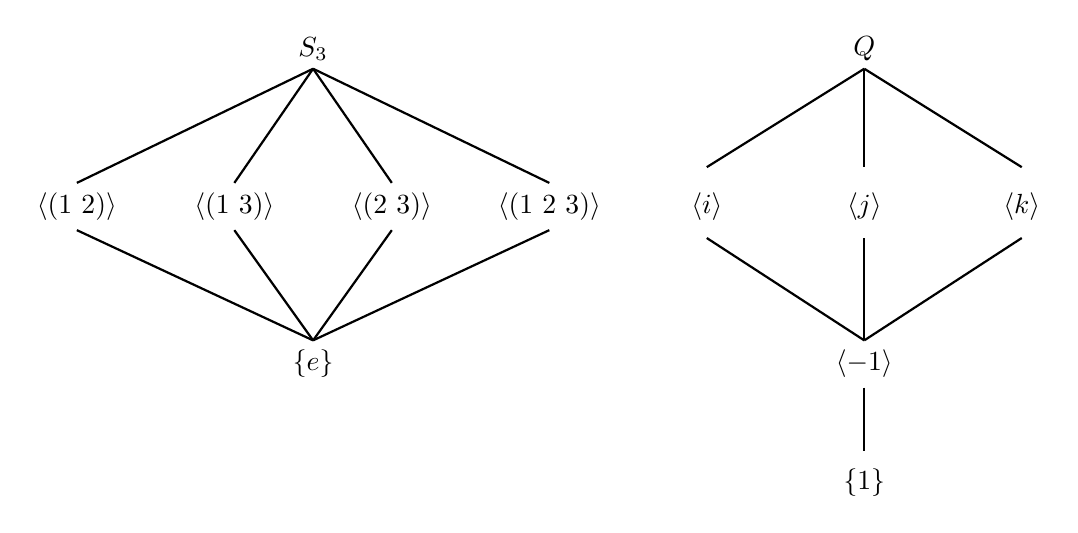
\begin{tikzpicture}[>=triangle 60]
    \coordinate (A) at (3,2.75);

    \coordinate (B) at (4,1.3);
    \coordinate (C) at (2,1.3);
    \coordinate (D) at (0,1.3);
    \coordinate (E) at (6,1.3);

    \coordinate (B') at (4,0.7);
    \coordinate (C') at (2,0.7);
    \coordinate (D') at (0,0.7);
    \coordinate (E') at (6,0.7);

    \coordinate (F) at (3,-0.7);

    \draw[thick] (A)--(B) node[midway,sloped,below] {};
    \draw[thick] (A)--(C) node[midway,sloped,below] {};
    \draw[thick] (A)--(D) node[midway,sloped,below] {};
    \draw[thick] (A)--(E) node[midway,sloped,below] {};

    \draw[thick] (F)--(B') node[midway,sloped,below] {};
    \draw[thick] (F)--(C') node[midway,sloped,below] {};
    \draw[thick] (F)--(D') node[midway,sloped,below] {};
    \draw[thick] (F)--(E') node[midway,sloped,below] {};

    \draw (3,3) node {$S_3$};

    \draw (4,1) node {$\langle (2\ 3) \rangle$};
    \draw (2,1) node {$\langle (1\ 3) \rangle$};
    \draw (0,1) node {$\langle (1\ 2) \rangle$};
    \draw (6,1) node {$\langle (1\ 2\ 3) \rangle$};

    \draw (3, -1) node {$\{ e \}$};

    \coordinate (Z) at (10,2.75);

    \coordinate (J) at (10,1.5);
    \coordinate (K) at (12,1.5);
    \coordinate (I) at (8,1.5);

    \coordinate (J') at (10,0.6);
    \coordinate (K') at (12,0.6);
    \coordinate (I') at (8,0.6);

    \coordinate (Q) at (10,-0.7);
    \coordinate (Q') at (10,-2.1);
    \coordinate (Q'') at (10,-1.3);

    \draw[thick] (Z)--(J) node[midway,sloped,below] {};
    \draw[thick] (Z)--(K) node[midway,sloped,below] {};
    \draw[thick] (Z)--(I) node[midway,sloped,below] {};

    \draw[thick] (J')--(Q) node[midway,sloped,below] {};
    \draw[thick] (K')--(Q) node[midway,sloped,below] {};
    \draw[thick] (I')--(Q) node[midway,sloped,below] {};

    \draw[thick] (Q'')--(Q') node[midway,sloped,below] {};

    \draw (10,3) node {$Q$};

    \draw (10,1) node {$\langle j \rangle$};
    \draw (8,1) node {$\langle i \rangle$};
    \draw (12,1) node {$\langle k \rangle$};
    \draw (10,-1) node {$\langle -1 \rangle$};

    \draw (10, -2.5) node {$\{ 1 \}$};
\end{tikzpicture}
\end{center}

\chapter{An Excursion: Subgroups of $\mathbf{Z}^+$}

We have built a complicated tower of definitions for us to comprehend without extensive use of examples. This aside is intended show the power of the concepts developed and to provide concrete usage of the abstractions developed. We will consider the additive integer group $\mathbf{Z}^+$. Before we begin, some more notation is useful. For a group with an operation $\circ$, with two subsets $S$ and $M$, define $S \circ M = \{ s \circ m : s \in S, m \in M \}$. For a single element $a$, define $a \circ M = \{ a \} \circ M$.

Now for any integer $a$, one can verify that $a\mathbf{Z}^+$ forms a subgroup of the integers. What is suprising is the following.

\begin{theorem}
    $G$ is a subgroup of $\mathbf{Z}^+$ if and only if $G$ is of the form $a\mathbf{Z}^+$ for some integer $a$.
\end{theorem}
\begin{proof}
    Let $G$ be a subgroup of $\mathbf{Z}^+$. If $G = \{ 0 \}$, then $G = 0\mathbf{Z}^+$. Otherwise, $G$ has some other non-zero element $a$. Thus $G$ contains a positive element, for $a$ is negative or positive, and if it is negative, then its inverse must be positive and contained in the subgroup by the closure property of a subgroup. By the well-ordering principle, $G$ contains a smallest positive element $b$. Using euclidean division, every element $c \in G$ is of the form $mb + n$, where $0 < n < b$. Now $n \in G$,  as $n = c - mb$, so we must conclude $n = 0$, as it cannot be a smaller positive integer than $b$. Thus every integer in $G$ is divisible by $b$, and every number divisible by $b$ is in $G$, so we conclude $G = b\mathbf{Z}^+$.
\end{proof}

Here are some common uses of these results in number theory:
\begin{itemize}
    \item For any numbers $a, b \in \mathbf{Z}^+$, $a\mathbf{Z}^+ + b\mathbf{Z}^+$ is a group. so it is equal to $c\mathbf{Z}^+$ for some integer $c$. It turns out $c$ is the greatest common denominator of $a$ and $b$, denoted $\gcd(a,b)$.
    \item Given $a,b \in \mathbf{Z}^+$, $a\mathbf{Z}^+ \cap b\mathbf{Z}^+$ is a subgroup of $\mathbf{Z}^+$, so it too is $c\mathbf{Z}^+$, and $c$ is the lowest common multiple of the two elements, denoted $\lcm(a,b)$.
\end{itemize}

Though we have focused only on $\mathbf{Z}^+$ in this aside, we note that the proofs can be applied to all cyclic groups, a concept we will define in the next chapter.

\chapter{Generators}

We begin with an interesting discovery on collections of subgroups.

\begin{lemma}
    Let $G$ be a group, and $(H_j)_{j \in \mathcal{J}}$ a family of subgroups. Then it follows that
    %
    \[ \bigcap_{j \in \mathcal{J}} H_j \]
    %
    is also a subgroup of $G$
\end{lemma}

Now let $G$ be a group, and $S$ a subset of that group. Take the set $\mathcal{M}$ to be the set of all subgroups of $G$ which contain $S$. Of course, $\mathcal{M}$ is non-empty as $G$ is a subgroup which contains $S$. Suppose we can index $\mathcal{M}$ completely by an index set $\mathcal{J}$. We make the following definition.

\begin{definition}
    Given a subset $S$ of a group $G$, we define the subgroup generated by $S$ to be the smallest subgroup that contains $S$, and we denote the subgroup $\langle S \rangle$. We call $S$ the {\bf generator} of the group $\langle S \rangle$. In the notation defined above this definition,
    %
    \[ \langle S \rangle = \bigcap_{j \in \mathcal{J}} \mathcal{M} \]
\end{definition}

Equivalently, the generated subgroup is the set of all elements of the form $x_1 x_2 \dots x_n$ where $x_i$ or $x_i^{-1}$ is in $S$. Any subgroup which contains $S$ must contain these elements, and these elements themselves from a subgroup of $G$. We write this subgroup as $\langle S \rangle$, and if $S$ is a finite group ordered by the sequence $\{ x_1, x_2, \dots, x_n \}$, we also write the subgroup as $\langle x_1, x_2, \dots, x_n \rangle$.

A simple example is taken from linear algebra. One standard theorem proven is that every invertible matrix is the product of elementary matrices. This means that $GL_n(\mathbf{F})$ is generated by the set of all elementary $n$ by $n$ matrices. It can be shown that this can be reduced to the set of all elementary matrices of the first and third kind.

If a group is generated by a single element, then the group is called cyclic. One example is $\mathbf{Z}^+$. Let $g$ be an element of a group $G$, and suppose that $\langle g \rangle$ is order $c$ for some natural number $c$. Then the following properties hold for $g$:

\begin{lemma} $\{ g, g^2, \dots, g^c \}$ are all distinct elements of $g$. \end{lemma}
\begin{proof}
    If $g^i = g^j$, for $0 < i < j \leq c$, then $g^{j-i} = e$. Then the smallest subgroup that contains $g$ is $\{ g, g^2, \dots g^{i-j} \}$,  hence the order of $g$ is $j-i < c$. By contradiction, $g^i \neq g^j$.
\end{proof}

\begin{corallary} For $k < c$, $g^k \neq e$ \end{corallary}
\begin{proof} For then $g^{k+1} = g$. \end{proof}

\begin{corallary} $g^c = e$. \end{corallary}
\begin{proof} $g^c$ is not any number from $g$ to $g^{c-1}$, so it must be the element of the group generated by $g$ that is different from the other elements before it. Thus $g^c = e$ by corallary (2.2.3), as no other element before $g^c$ is $e$. \end{proof}

\begin{lemma} $g^k = e$ if, and only if, $c|k$ \end{lemma}
\begin{proof} This is left to the reader. It is a simple application of euclidean division used previously in our discussion of $\mathbf{Z}^+$.
\end{proof}

\begin{lemma} If $\langle g \rangle$ is infinite, then $g^i \neq g^j$ if $i \neq j$. \end{lemma}
\begin{proof}
    If $g^i = g^j$ for some $i > j$, then $g^{i-j} = e$, showing the cyclic group is at most order $i - j$.
\end{proof}

We have also shown that in $\mathbf{Z}^+$ that every subgroup is cyclic, but this proof can be easily extended to the following: every subgroup of a cyclic group is cyclic. We leave it to the reader to use the techniques of the excursion to establish this.

Given an element $g$ in an arbitrary group $G$, we define the order of $g$ to be the order of the group $\langle g \rangle$. Of course, if $\langle g \rangle$ is finite, this is exactly the least positive integer $a$ such that $g^a = e$.

\begin{lemma} The order of an element $ab$ is the same as the order of an element $ba$. \end{lemma}
\begin{proof}
    Consider the group $\langle ab \rangle$.
    $(ba)^{-1} = a^{-1}b^{-1}$.
    Suppose the order of $ab$ is finite, of order $k$. Then $(ab)^k = e$, which means that $b(ab)^k = b$, and $b(ab)^k = (ba)^k b$, so that $(ba)^k b = b$, and thus $(ba)^k = e$. Thus the order of $(ba)$ is less than or equal to the order of $(ab)$. This process can be done backwards to determine that the order of $(ab)$ is less than or equal to the order of $(ba)$, so the two are equal.
\end{proof}

\chapter{Homomorphisms}

Another way we can understand objects that we don't understand is by connecting metaphors between those objects that we do. We can formalize this in a group with the concept of a homomorphism

\begin{definition}
Let $G$ be a group with operation $\circ$ and $H$ a group with operation $*$. A {\bf homomorphism} between $G$ and $H$ is a function $f$ such that for any elements $x$ and $y$. $f(x \circ y) = f(x) * f(y)$. We say that $G$ and $H$ are homomorphic. If a homomorphism is bijective, we call it an isomorphism. If $G = H$, we call a homomorphism an endomorphism, and an isomorphism an automorphism.
\end{definition}

What a homomorphism means intuitively is that information about the group $G$ can be implanted into a subgroup of $H$. Some elements may become one element, but the information is still there. An isomorphism states that all algebraic information about $G$ holds in $H$ -- effectively, they are the same group with different names for the operations and elements of the group.

\begin{definition}
    The {\bf kernel} of a homomorphism $\varphi$, denoted $\ker(\varphi)$ is the set of elements in the domain that are mapped to the identity element in the range.
\end{definition}

The following properties hold for any homomorphism $\varphi$:

\begin{lemma} $\varphi(e) = e$ \end{lemma}
\begin{proof} $\varphi(e) = \varphi(ee) = \varphi(e)\varphi(e)$, hence $\varphi(e)$ is idempotent. \end{proof}

\begin{lemma} $\varphi(a^{-1}) = \varphi(a)^{-1}$. \end{lemma}
\begin{proof} $\varphi(a^{-1})\varphi(a) = \varphi(aa^{-1}) = \varphi(e) = e$. \end{proof}

\begin{lemma} The kernel of a homomorphism is a subgroup \end{lemma}
\begin{proof} If $\varphi(a) = e$ and $\varphi(b) = e$, $\varphi(a^{-1}) = \varphi(a)^{-1} = e^{-1} = e$ so that $\varphi(a^{-1}b) = e$. \end{proof}

\begin{lemma} The image of a homomorphism is a subgroup \end{lemma}
\begin{proof} If $a$ is a group element such that $\varphi(x) = a$ for some elements $a$ and $x$, then $\varphi(x^{-1}) = a^{-1}$, and if $b$ is an element such that $\varphi(y) = b$ for some element $y$, then $\varphi(x^{-1}y) = a^{-1}b$. \end{proof}

\begin{lemma} A homomorphism is injective if and only if $\varphi(a) = e$ implies $a = e$. \end{lemma}
\begin{proof} We prove both implications.\\
$(\Rightarrow)$ If a homomorphism is injective, and if $\varphi(a) = e$, then $a = e$ as $\varphi(e) = e$.\\
$(\Leftarrow)$ If $\varphi(a) = e$ implies $a = e$, then if $\varphi(a) = \varphi(b)$, then $\varphi(ab^{-1}) = e$, so that $ab^{-1} = e$ and thus $a = b$.
\end{proof}

Some examples of homomorphisms are the following:
\begin{itemize}
    \item The determinant function from $GL_n(\mathbf{F}) \to \mathbf{F}^\times$
    \item The exponentiation map $x \mapsto e^x$
    \item For any element $a$ in $G$, the map from $\mathbf{Z}^+$ defined by $x \mapsto a^x$.
    \item The absolute value map from $\mathbf{C}^\times$ to $\mathbf{R}^\times$
\end{itemize}
 
For a group, the set of automorphisms on the group, taken with the operation of composition of functions, form a group. Given an element $g$ in $G$, the set of automorphisms $h \mapsto ghg^{-1}$ defines the set of inner automorphisms, a subgroup of the set of automorphisms. The map that sends $g$ to its inner automorphism is a homomorphism. The kernel of this homomorphism is the center group

\[Z(G) = \{ g \in G : \forall h: gh = hg \}\]

\chapter{Cosets}

We were previously introduced to subgroups as an attempt to understand the group as a sum of its parts. Cosets are another way to do this.

\begin{definition}
    Let $H$ be a subgroup of a group $G$. Define an equivalence relation $\sim$ by $x \sim y$ if $x \in yH$. The equivalence classes formed by the relation are denoted $G/H$ and pronounced as `$G$ modulo (mod) $H$'. Each equivalence class is called a {\bf left coset}.
\end{definition}

\begin{lemma}
    Every left coset is of the form $gH$ for some element $g$ that is in the equivalence class.
\end{lemma}
\begin{proof}
    Let $C$ be an arbitrary equivalence class in $G/H$. Then $C$ is non-empty; there is some element $g$ in the class. We know $gH \subseteq C$, as for any element $h \in H$, $g \sim gh$. But also $C \subseteq gH$, as if $g \sim c$ for some $c \in C$, $c \in gH$.
\end{proof}

Right cosets are defined equivalently in the obvious way, by the equivalence relation $g ~ k$ if $g \in Hk$. Like left cosets, all right cosets can be written $Hg$ for some $g$. Whether we use left cosets or right coses does not matter, theorems can be proved in equal power for each. The theorem below shows that there is actually a close connection between the two coset types.

\begin{lemma} There is a one to one correspondence between left cosets and right cosets of any group \end{lemma}
\begin{proof}
Let $G$ be a group, and $H$ a subgroup that generates $G/H$. Consider the mapping from left cosets to right cosets defined by $gH \mapsto Hg^{-1}$. We claim this mapping is a function. Suppose for two elements $g$ and $g'$ in $G$, $gH = g'H$. Then $gh = g'h'$ for some elements $h$ and $h'$ in $H$. But then, it follows that $(gh)^{-1} = (g'h')^{-1}$, which when evaluated gives us the equation $h^{-1}g^{-1} = h'^{-1}g'^{-1}$. We rearrange to get that $g^{-1} = hh'^{-1}g'^{-1}$. By the property of closure in a group, $hh'^{-1} \in H$, so that $g^{-1} = h''g'^{-1}$ for $h'' = hh'$. This means precisely that $g^{-1} \in Hg'^{-1}$, but also $g^{-1} \in Hg^{-1}$ (simply take $e \in H$). As cosets partition the group, we must conclude that $Hg^{-1} = Hg'^{-1}$. The two are equal, as was desired. In addition to this, the map is a bijection, with an inverse function defined by $Hg \mapsto g^{-1}H$. Thus we have a one-to-one correspondence, as was required.
\end{proof}

The number of cosets (whether left or right) in $G/H$ is denoted $(G:H)$, and is called the index of $H$ in $G$.

We now come to one of the most important theorems in basic group theory, named after one of the pioneers of group theory, the french mathematician Joseph-Louis-Lagrange. It gives a useful characteristic of all subgroups of a finite group. Though the statement is formidible, the mechanics we have built up make the proof relatively simple -- our definitions were the hard part to understand.

\begin{theorem}[Lagrange's Theorem]
    The order of a subgroup of a finite group divides the order of the entire group.
\end{theorem}
\begin{proof}
Let $G$ be a finite group, and $H$ a subgroup. Let $g$ and $g'$ be arbitrary elements of $G$. Define a function from $gH$ to $g'H$ defined by $a \mapsto g'g^{-1}a$. This mapping is bijective, as it has an inverse function defined by the mapping $b \mapsto gg'^{-1}b$. Thus the order of one coset is equal to the other coset. We obtain the following correspondence: for any coset $gH$, $|G| = |gH|(G:H)$. What this means that if any two of the three elements is finite, so is the third, and the equation holds. By noting that $H$ is a coset (simply take the coset of $e$), we obtain Lagrange's theorem as a corallary, $|G| = |H|(G:H)$, so $|H| \divides |G|$.
\end{proof}

Lagrange did not completely prove the theorem, showing it only for subgroups of the symmetric groups. The first complete theorem was published by Gauss in 1801.

\begin{corallary}[The Multiplicative Property]
    Let $G$ be a group, $H$ a subgroup of $G$, and $M$ a subgroup of $H$. Then $(G:M) = (G:H)(H:M)$.
\end{corallary}
\begin{proof}
    If $M$ is a subgroup of $H$, Lagrange's theorem tells us that $|H| = |M|(H:M)$. By further application of (1.4.2), It then follows that $|G| = |H|(G:H) = |M|(G:H)(H:M)$. Noticing that $M$ is also a subgroup of $G$, $|G| = |M|(G:M)$. We conclude $|M|(G:M) = |M|(G:H)(H:M)$ By dividing by $|M|$ (which is non-zero as $M$ is non-empty), we obtain the fact that $(G:M) = (G:H)(H:M)$.
\end{proof}

We now harken back to the beginning of the book. We said that Euler used the ideas of Lagrange to prove his theorem of the totient function (Look back to the first chapter if you don't remember). We now have the power to prove this as a corallary.

\begin{corallary}[Euler's Theorem]
    For any two relatively prime integers $a$ and $b$,
    %
    \[ a^{\varphi(b)} \equiv 1 \mod{b} \]
\end{corallary}
\begin{proof}
    Consider the set $P$ of relatively prime integers to $b$, with the operation of multiplication. We show that, modulo $b$, this set forms a group. Let $x$ be a number relatively prime to $b$. Then there exists integers $m$ and $n$ such that $mb + nx = 1$, so that $mb \equiv 1 \mod{b}$. Furthermore, if for some number $x$ there exists a number $y$ such that $xy \equiv 1 \mod{b}$, then $xy + mb = 1$ for some number $m$. It follows that the greatest common denominator of $x$ and $b$ must be 1, so the two are relatively prime. Finally, if $x$ and $y$ are relatively prime to $b$, so is $xy$, because the two numbers share no prime factors. Thus we conclude that the elements in $P$ modulo $b$, denoted $P/b\mathbf{Z}^\times$ (cosets of the multiplicative group $b\mathbf{Z}^\times$) form a group under multiplication. $a$ modulo $b$ is a member of this group. Take the subgroup $\langle a \rangle$, which must be a finite order, which we denote by $k$. Since the set contains $\varphi(b)$ elements, we have that $k \divides \varphi(b)$ by Lagrange's theorem. But then $a^{\varphi(b)} \equiv 1 \mod{b}$ by (5.0.20).
\end{proof}

\chapter{Normal Subgroups}

\begin{theorem}[Characterization of Normal Subgroups]
Let $H$ be a subgroup of a group $G$. The following statements are equivalent, and if any hold, we say $H$ is normal in $G$ and write $H \lhd G$:
\begin{enumerate}
    \item $gHg^{-1} \subseteq H$ for all $g$
    \item $gHg^{-1} = H$ for all $g$
    \item $gH = Hg$ for all $g$
    \item For all $g$, there is $g'$ such that $gH = Hg'$
\end{enumerate}
\end{theorem}
\begin{proof}
    First we show (1) is equivalent to (2). Suppose $ghg^{-1} \subseteq H$ for all $g$. Then $gH \subseteq Hg$ (multiply both sides of the relation on the right by $g$. But also $g^{-1}Hg \subseteq H$, such that $Hg \subseteq gH$, so that $Hg = gH$. The reverse is obvious. We obtain (3) from (2) by multiplying both sides of the equation on the right by $g$, and the reverse by multiplying on the right by $g^{-1}$. The implication from (3) to (4) is obvious. From (4), note if $gH = Hg'$, $ge = g \in Hg'$, so that $Hg' = Hg$ as cosets are equal or disjoint. Thus all statements are shown to be equivalent.
\end{proof}

We use normal subgroups along with homomorphisms to connect groups. To tease this, we show the following theorem.
\begin{theorem} The kernel of a homomorphism is a normal subgroup \end{theorem}
\begin{proof} Let $G$ and $H$ be groups, and $\varphi$ a homomorphism between $G$ and $H$. If $\varphi(j)=e$, $\varphi(gjg^{-1}) = \varphi(g)\varphi(j)\varphi(g)^{-1} = \varphi(g)\varphi(g)^{-1} = e$. Thus $gjg^{-1}$ is in the kernel for any element $g$ in $G$, and we have shown (1) in the definition. \end{proof}

The trivial group is always normal, because given any element $g$, $g^{-1}eg = g^{-1}g = e$. Furthermore, for any group $G$, $G \lhd G$ (we leave this to the reader to verify). Thus no group posesses that characteristic that it contains no normal subgroups. Thus we must define a property along these lines in a slightly more precise way. A group is simple if it contains no non-trivial normal subgroups, that is, if the only normal subgroups are $\{ 0 \}$ and the group itself.

Some examples of normal subgroups are the following. Verification of normality is left as an exercise:
\begin{itemize}
    \item If $G$ is abelian, and $H$ is a subgroup, $H \lhd G$.
    \item $SL_n(\mathbf{F}) \lhd GL_n(\mathbf{F})$
    \item If $H$ is a subgroup of $G$ of index two, $H \lhd G$
    \item If a group $G$ is normal, and $H$ is a cyclic subgroup, for any subgroup $I$ in $H$, $I \lhd G$.
\end{itemize}

\chapter{Isomorphism Theorems}

We can finally use coset constructions to prove something meaningful. Let $G$ be a group and $H$ a normal subgroup. For two cosets $M$ and $N$ in $G/H$, define an operation $M \circ N = MN$. As $M = gH$ and $N = g'H$ for some $g,g' \in H$, $MN = gHg'H = gg'HH = gg'H$. Thus the operation is closed in $G/H$, and $G/H$ forms another group: the product or factor group. $H$ is the identity in this group. The map $g \mapsto gH$ is the canonical map or projection $\pi$ from $G$ to $G/H$, and is a surjective homomorphism (note this shows that any normal subgroup is the kernel of some homomorphism). The projection of $G$ onto $G/H$ has a property that we prove in a more general form.

\begin{theorem}[The First Isomorphism Theorem]
Let $\varphi$ be a homomorphism between two groups $G$ and $H$, and let $N$ be a normal subgroup of the kernel of $\varphi$. Then there is a homomorphism $\overline{\varphi}$ from $G/H$ to $H$ such that $\overline{\varphi} \circ \pi = \varphi$, where $\pi$ is the canonical map. If $N$ is the kernel, the map $\overline{\varphi}$ is an isomorphism to $\im(\varphi)$.
\end{theorem}
\begin{proof}
    For every $n \in N$, we have $\varphi(n) = e$ as $N$ is a subgroup of the kernel. Thus if $gN = hN$ for $g,h \in G$, $\varphi(g) = \varphi(h)$. The map $\overline{\varphi}: gN \mapsto \varphi(g)$ then becomes well defined. It is a homomorphism as $gHhH = ghH$, so $ghH$ is mapped to $\varphi(gh) = \varphi(g)\varphi(h)$. We then obtain that $\overline{\varphi} \circ \pi = \varphi$ by construction. Because $\pi$ is surjective, the map is unique.

    Now if $N$ is the kernel, the homomorphism is injective. $\varphi(a) = \varphi(b)$ implies $\varphi(ab^{-1}) = e$. Then $ab^{-1} \in N$, and $ab^{-1}N = N$, but as $N$ is normal, it is also true that $ab^{-1}N = aNb^{-1}$, so that $aNb^{-1} = N$, and thus $aN = Nb = bN$. What this says is that, if $\overline{\varphi}(aN) = \overline{\varphi}(bN)$, then $aN = bN$, so the map is injective. The map is of course surjective onto its image, so the map is an isomorphism.
\end{proof}

\begin{wrapfigure}{1}{3.5cm}
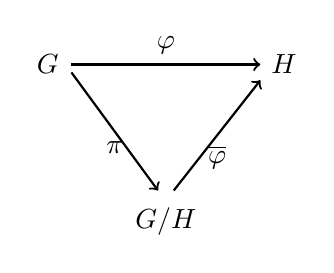
\begin{tikzpicture}[description/.style={fill=white,inner sep=2pt}]
\coordinate (A) at (0.3,1.5);
\coordinate (B) at (2.7,1.5);
\coordinate (C) at (1.4,-0.1);
\coordinate (D) at (1.6,-0.1);
\coordinate (E) at (2.7,1.3);
\coordinate (F) at (0.3,1.4);

\draw (0,1.5) node {$G$};
\draw (3,1.5) node {$H$};
\draw (1.5,-0.5) node {$G/H$};

\draw[thick,->] (A)--(B) node[midway,above] {$\varphi$};
\draw[thick,->] (F)--(C) node[midway,below] {$\pi$};
\draw[thick,->] (D)--(E) node[midway,below] {$\overline{\varphi}$};

\end{tikzpicture}
\end{wrapfigure}

It is convenient here to introduce the concept of a commutative diagram. A commutative diagram is a directed graph where vertices are sets and edges are functions between the sets it connects, with the following property. If there are two paths
%
\begin{align*}
    S \xrightarrow{f_1} A_1 \xrightarrow{f_2} \dots \xrightarrow{f_{n-1}} A_n \xrightarrow{f_n} E\\
    S \xrightarrow{g_1} B_1 \xrightarrow{g_2} \dots \xrightarrow{g_{m-1}} B_m \xrightarrow{g_m} E
\end{align*}
from $S$ to $E$, then $f_n \circ \dots \circ f_1 = g_m \circ \dots \circ f_1$. An example diagram is to the upper right, representing the functions in the first isomorphism theorem.

A simple application of the first isomorphism theorem is a way to completely understand the cyclic groups, a classification. The relation on groups $x \sim y$ if $x \equiv y$. In algebra, we refer to a classification of groups as a set of isomorphism classes for those groups. It is the ultimate achievement as it allows us to show that these are the only way the operations can perform.

\begin{theorem}[The Classification of Cyclic Groups]
    Every cyclic group is isomorphic to either $\mathbf{Z}$ or $\mathbf{Z}/n\mathbf{Z}$ for some integer $n$.
\end{theorem}
\begin{proof}
Let $\langle g \rangle$ be a cyclic group. Define a surjective homomorphism from $\mathbf{Z}^+$ to $\langle g \rangle$ by the mapping $r \mapsto g^r$. If $\langle g \rangle$ is order $n$, $n\mathbf{Z}^+$ is the kernel of the map. Then $\langle g \rangle \cong \mathbf{Z}^+/n\mathbf{Z}^+$ by the first isomorphism theorem. If $\langle g \rangle$ is infinite, the kernel of the map is $\{ 0 \}$, and $\mathbf{Z}^+/0\mathbf{Z}^+ \cong \mathbf{Z}^+$, so $\langle g \rangle \cong \mathbf{Z}^+$.
\end{proof}

We have a trilogy of isomorphism theorems to show. Here is the second.


\begin{center}
\begin{tikzpicture}
    \coordinate (Z) at (1.9,-2.75);
    \coordinate (Z') at (2.1,-2.75);

    \coordinate (J) at (2,-1.5);
    \coordinate (K) at (4,-1.5);
    \coordinate (I) at (0,-1.5);

    \coordinate (J') at (2,-0.6);
    \coordinate (K') at (4,-0.6);
    \coordinate (I') at (0,-0.6);

    \coordinate (Q) at (2,0.7);
    \coordinate (Q') at (2,2.1);
    \coordinate (Q'') at (2,1.3);

    \draw[thick,->] (K)--(Z') node[midway,sloped,below] {};
    \draw[thick,->] (I)--(Z) node[midway,sloped,below] {};

    \draw[thick,->] (Q)--(K') node[midway,sloped,below] {};
    \draw[thick,->] (Q)--(I') node[midway,sloped,below] {};

    \draw[thick,->] (Q')--(Q'') node[midway,sloped,below] {};

    \draw (2,-3) node {$H \cap N$};

    \draw (0,-1) node {$H$};
    \draw (4,-1) node {$N$};
    \draw (2,1) node {$HN$};

    \draw (2, 2.5) node {$G$};
\end{tikzpicture}
\end{center}

\begin{theorem}[The Second Isomorphism Theorem]
    Let $G$ be a group, and $N$ and $H$ subgroups such that $N \lhd G$. The $NH$ is a subgroup of $G$, and $N \cap H \lhd G$. The assignment map $h(N \cap H) \mapsto hN$ is an isomorphism, and so $H/N \cap H \cong NH/H$:
\end{theorem}
\begin{proof}
    First we prove $NH$ is a subgroup. If $n_1h_1$ and $n_2h_2$ are in $NH$, then $n_1h_1(n_2h_2)^{-1}$ is in $NH$ by the following calculation:

    \begin{align*}
    n_1h_1(n_2h_2)^{-1} &= n_1h_1h_2^{-1}n_2^{-1}\\
    &= n_1((h_1h_2^{-1})n_2^{-1}(h_1h_2^{-1})^{-1})h_1h_2^{-1}
    \end{align*}

    The equation above is in $NH$ as $N$ is normal, so that $(h_1h_2^{-1})n_2^{-1}(h_1h_2^{-1})^{-1}$ is in $N$. The map $h \mapsto hN$ is a surjective homomorphism from $H$ to $NH/N$, and the kernel is $N \cap H$ (so $N \cap H$ is normal), and $H/N \cap H \cong NH/N$ by the first isomorphism theorem.
\end{proof}

The final isomorphism theorem is the following.

\begin{theorem}[The Third Isomorphism Theorem]
    Let $M$ and $N$ are normal subgroups of a group $G$, where $N$ is also a normal subgroup of $M$. Then $M/N$ is a normal subgroup of $G/N$, and $(G/N)/(M/N) \cong G/M$.
\end{theorem}
\begin{proof}
    Define an assignment from $G/N$ to $G/M$ by $gN \mapsto gM$. It is a surjective homomorphism, well defined as $N$ is a subgroup of $M$, so that $gN \subseteq gM$ for any $g$. The kernel of this map are all sets of elements $gN$ such that $gM = M$, which is precisely the elements $g$ that are elements of $M$. Then the kernel is $M/N$ (a normal subgroup), so by the first isomorphism theorem, we obtain that $(G/N)/(M/N) \cong G/M$.
\end{proof}

Surprise, turns out we have another isomorphism theorem.

\begin{theorem}[The Lattice/Fourth Isomorphism Theorem]
Let $G$ be a group, and $N$ a normal subgroup. Then there is a bijection $f$ from subgroups of $G$ which contain $N$ to subgroups of $G/N$ such that $f(H)$ is denoted $\overline{H}$. The bijection has the following properties for any two subgroups $H$ and $K$:

\begin{itemize}
    \item $H \subset K$ if and only if $\overline{H} \subset \overline{K}$.
    \item If $H \subset K$, $(H:K) = (\overline{H}:\overline{K})$.
    \item $\overline{\langle H, K \rangle} = \langle \overline{H}, \overline{K} \rangle$
    \item $\overline{A \cap B} = \overline{A} \cap \overline{B}$
    \item $H \lhd K$ if and only if $\overline{H} \lhd \overline{K}$
\end{itemize}
\end{theorem}
\begin{proof}
    Given a subgroup $H$ of $G$ which contains $N$, define a mapping by $H \mapsto H/N$. The properties above can (and should be) be checked by the reader.
\end{proof}

\chapter{The Symmetric Group}

The symmetric group was previously defined as the set of permutations on a set. In the context of an example, this group seems just a trivial example. This is not so. One reason why the group is generally interesting is Cayley's theorem, which relates the set of groups to all other groups.

\begin{theorem}[Cayley's Theorem]
    Every group is isomorphic to a subgroup of a symmetric group:
\end{theorem}
\begin{proof}
    Let $G$ be a group. For each $g \in G$, define a permutation $\pi_g$ on the group defined by the map $h \mapsto gh$. The function is a permutation as it is bijective -- there is an inverse function $h \mapsto g^{-1}h$. The map from the group to its permutation is a homomorphism as for any two elements $g$ and $g'$ $\pi_g \circ \pi_{g'} = \pi_{gg'}$. Furthermore, the homomorphism is injective, as if $\pi_g = \text{id}$, then $gh = h$ for all elements $h$, and for any specific one, we obtain that $g = e$. Thus $G$ is isomorphic to the image of the permutation map, which is a subgroup of $S_{|G|}$.
\end{proof}

From Cayley's theorem, it follows that anything algebraically we prove about the subgroups of symmetric groups follows for all groups by the isomorphism property. Thus we will spend the rest of this chapter focusing on the components that form the symmetric group.

\begin{definition}
    Given a set $M$ and a permutation $\pi$ on $M$, the {\bf support} of $\pi$, denoted $\sup(\pi)$, is equal to $\{ m \in M : \pi(m) \neq m \}$. A cycle of length $k$ is a permutation $\pi$ such that $|\sup(\pi)| = k$, and such that we can order $\sup(\pi)$ to be $(x_1, x_2, \dots, x_k)$ in a way that $\pi(x_n) = x_{n+1 \mod k+1}$. A cycle of length two is called a transposition.
\end{definition}

We write the function $\pi$ as $(x_1, \dots, x_k)$. If $\sigma$ and $\tau$ are two permutations, such that $\sup(\sigma) \cap \sup(\tau) = \emptyset$, $\sigma \circ \tau = \tau \circ \sigma$. This is because the two act independently on the set they permute.

\begin{theorem}
Every permutation on a finite non-empty set which is not the identity can be written as the product of cycles with disjoint support. This is unique up to reordering:
\end{theorem}
\begin{proof}
    We prove this theorem by induction. For a one element set, the proof is vacously true. Now suppose that permutations on sets of less than $n$ elements can be written as disjoint cycles. Consider a set $X$ of $n$ elements. Take an arbitrary element $x_1$. Then form a sequence $(x_1, \pi(x_1), \pi^2(x_1), \dots, \pi^n(x_1)$. Such that $\pi^{n+1}$ is the least function for which $\pi^{n+1}(x_1) = x_1$. This is always possible in a finite set by an easy application of the pidgeonhole principle. Denote these elements as the sequence $(x_1, x_2, \dots, x_n)$. Then $\pi|_{\{ x_1, \dots, x_n\}}$ is a cycle of length $n$. Now $X - \{ x_1, \dots, x_n \}$ is a set of less than $n$ elements, so that we can decompose it $\pi|{\{ x_1, \dots, x_n\}}$ into a product of disjoint cycles. Then, since the support of each is disjoint,
    $\pi|_{\{ x_1, \dots, x_n\}} \circ \pi|{\{ x_1, \dots, x_n\}} = \pi$, and $\pi$ is a product of disjoint cycles.
\end{proof}

\begin{lemma}
    Let $\pi \in S_X$ and $\sigma = (x_1\ x_2\ \dots\ x_n)$. Then it follows that
    \[\pi \sigma \pi^{-1} = (\pi(x_1)\ \pi(x_2)\ \dots\ \pi(x_n))\]
\end{lemma}
\begin{proof}
    This follows as $\pi \sigma \pi^{-1} (\pi(x_i)) = \pi \sigma(x_i) = \pi(x_{i+1})$. If $x \notin \sup(\sigma)$, then $\pi \sigma \pi^{-1} (\pi (x)) = (\pi \sigma) (x) = \pi(x)$, so that $\pi(x) \notin \sup(\pi \sigma \pi^{-1})$.
\end{proof}

\begin{lemma}
    Any symmetric group is generated by the set of transpositions in that group.
\end{lemma}
\begin{proof}
Each cycle can be decomposed into transpositions. Concretely, this is the fact that
%
\[ (x_1\ \dots\ x_n) = (x_1\ x_n) (x_1\ x_{n-1}) \dots (x_1\ x_2) \]
%
We have shown that $S_X$ is generated by the set of cycles, hence $S_X$ is generated by the set of transpositions.
\end{proof}

The parity or signum of a permutation $\pi$ is based on the number of transpositions that is is composed of. If the number is even the value is $1$, else it is $-1$. We show that it this definition is well defined.

\begin{lemma}
    Any two compositions of transpositions that are equal either both have an even number of transpositions or both have an odd number.
\end{lemma}
\begin{proof}
    Let $(\sigma_1\ \sigma_2\dots\sigma_n) = (\pi_1\ \pi_2\dots\pi_m)$, where each composition is a sequence of transpositions. Every transposition can be written as a product of odd number of transpositions of adjacent elements, i.e
    %
    \[ (n\ m) = (n\ n+1)(n+1\ n+2)\dots(m-1\ m)(m-1\ m-2)\dots(n+1\ n) \]
    %
    Now decompose each transposition into a product of adjacent elements like above. We get a new sequence, that $(\sigma'_1\ \sigma'_2\dots\sigma'_{n'}) = (\pi'_1\ \pi'_2\dots\pi'_{m'})$. Now if we multiply from left to right the new sequence of the left with the old sequence, we obtain the fact that $n - n'$ and $m - m'$ are even. If we do this on the left of the right sequence with the left, we get that $m' - n'$ is even. Hence $m' - n$ is even, and so $m - m'$ is even, which is what we wanted to show.
\end{proof}

The parity operation defines a homomorphism from $S_n$ into $\mathbf{Z}^\times$. The kernel of this is $A_n$, the alternating group, a normal subgroup of $S_n$. Here are some properties of $A_n$.

\begin{lemma} If $\tau$ is a transposition, $S_n = A_n \cup \tau A_n$. Thus $A_n = n!/2$. \end{lemma}

\begin{lemma} $A_n$ is generated by the set of all three cycles \end{lemma}
\begin{proof}
    We need only prove that the product of two arbitrary transpositions $(a\ b)$ and $(c\ d)$ is generated by three cycles. If $\sup(a\ b) \cap \sup(c\ d) = \emptyset$, $(a\ b)(c\ d) = (a\ c\ b)(a\ c\ d)$. Otherwise without loss of generality, we may consider $a = c$. If $b = d$, then $(a\ b)(c\ d) = \mathbf{1}$. If $b \neq d$, $(a\ b)(c\ d) = (a\ b)(c\ d) = (c\ b\ a)$. Since $A_n$ is generated by pairs of transpositions, it is generated by three cycles.
\end{proof}

Saving the hardest for last:

\begin{lemma} $A_n$ is simple when $n \neq 4$ \end{lemma}
\begin{proof}
    This proof is about a page long. I will write it later.
\end{proof}

The fact that $A_4$ is not simple results in far reaching ramifications in Galois theory, where it implies that there is no formula for finding the roots of quintic polynomial roots.

\chapter{Group Actions}

Automorphisms are symmetries on a group, which, when taken together, form a group as a whole. The symmetry group acts as a more general notion of symmetries of a set. Through these actions, we obtain large amounts of information about both the group and the set. These are specific notions of a more general structure that we now describe, a group action.

\begin{definition}
A {\bf group action} on a set $G$ and set $X$ is a homomorphism from $G$ to $S_{|X|}$. As each $g \in G$ has an associated permutation, for $x \in X$ we write $gs$ for the permutation associated with $g$ acting on $s$. We call $X$ a {\bf G-set}.
\end{definition}

It is simple to show $g(hx) = (gh)x$ and $ex = x$, for $g,h,e \in G$ and $x \in X$. Another way of saying the first part of the statement is that, if $\varphi$ is the homomorphism defining the action, $\varphi(g) \circ \varphi(h) = \varphi(gh)$, and the section is saying that $\varphi(e) = \mathbf{1}$. This is just a definition of a homomorphism from a group to the symmetric group, so is van equivalent way of defining a group action.

\begin{definition}
Given a group $G$, and a $G$-set $S$, for $s \in S$, let the {\bf orbit} of $s$ be $Gs$, the set of all $gs$ for $g \in G$.
\end{definition}

The relation $x \sim y$ if $Gx = Gy$ is an equivalence relation and partitions the set into orbits of $S$. Note that this means the group acts independently on each of a $G$-set's orbits.

\begin{definition}
    A $G$-set is transitive if it has just one orbit.
\end{definition}

This just means that for any two elements $x$ and $y$ in a $G$-set $X$, there is some $g \in G$ such that $gx = y$.

\begin{definition}
    An action is faithful if the homomorphism defining it is injective.
\end{definition}

\begin{definition}
    A map $\alpha$ from a  $G$-set $X$ to a $G$-set $Y$ is a $G$-morphism if $\alpha(gx) = g\alpha(x)$ for all $g \in G$ and $x \in X$. $\alpha$ is an isomorphism if it is bijective.
\end{definition}

To relate this concept back to concepts previously talked about, a $G$-morphism is sort of like an isomorphism between $G$-sets. $G$-sets have no operation defined to compose them, however, so we must use the group action to define the isomorphism.

\begin{definition}
    An element $x$ in a $G$-set $X$ is a {\bf fixed point} if $gx = x$ for every $g \in G$. The set of all fixed points is denoted $X^G$.
\end{definition}

\begin{definition}
    Given any $x \in X$, $G_x = \{ g \in G : gx = x \}$ is a subgroup called the isotropy subgroup of $x$ in $G$.
\end{definition}

As an example, let $G$ act on itself by conjugation, that is, $g(h) = ghg^{-1}$. The isotopy subgroups are called centralizers $C_G(h) = \{ g \in G : gh = hg \}$. A fixed point is called a center, and the set of all centers is denoted $Z(G)$, which we have previously shown as the center group.

As another example, consider conjugation from $G$ on its subgroups. Then the isotropy group of a subgroup $H$ is the normalizer $N_G(H)$, which is the set $\{ g \in G : gHg^{-1} = H \}$. The fixed points of this transformation are precisely the normal subgroups.

Consider the group $SL_n(\mathbf{R})$ acting on the upper half of the complex plane, that is, the set $\{ z \in \mathbf{C} : \im(z) > 0 \}$ by the mobius transform below:

\[\begin{pmatrix} a & b \\ c & d \end{pmatrix} z = \frac{az + b}{cz + d}\]

The isotropy subgroup of $i$ is the special orthogonal group $SO(2)$, the set of matrices with orthonormal columns. The mobius transform is transitive. A meromorphic function on $H$ invariant under $SO(2)$ is called a modular function, and is essential to the study of number theory, string theory, and the study of monstrous moonshine.

\chapter{Direct Products, Semiproducts, and Abelian Groups}

Let $I$ be an index set, and $\{ G_i \}_{i \in I}$ a family of groups. Then the direct product of $\{ G_i \}$, denoted $\bigtimes_{i \in I} G_i$, is a group with operation $\bigtimes_{i \in I} g_i \circ \bigtimes_{i \in I} h_i = \bigtimes_{i \in I} g_ih_i$. The group is called the product group.

Let $r$ and $s$ be two relatively prime integers. Suppose $G$ is a cyclic group of order $rs$. Then $G$ is isomorphic to the direct product of cyclic groups $R$ and $S$, where $R$ is order $r$ and $S$ is order $s$.
\begin{proof}
    $R \times S$ is a cyclic group generated by $(x,y)$, where $x^r = e$, and $y^s = e$. This follows as $(x,y)^{rs} = (x^{rs},y^{rs}) = (e,e)$. If $(x,y)^m = (x^m,y^m) = (e,e)$, $r|m$ and $s|m$, so $rs|m$.
\end{proof}

Let $H$ and $K$ be normal subgroups of a group $G$, such that $H \cap K = \{ e \}$, and $HK = G$. Then $H \times K \cong G$:
\begin{proof}
    Define a map $(h,k) \mapsto hk$. The map is bijective, as $HK = G$, and if $hk = e$, $h = k^{-1}$, so $k^{-1} \in H$, so $k = h = e$. $hkh^{-1} \in K$, as $K$ is normal, but it is also in $N$ as $N$ is normal, hence $hkh^{-1}k^{-1} = e$, so $hk = kh$, and thus the map is a homomorphism as $h_1k_1h_2k_2 = h_1h_2k_1k_2$.
\end{proof}

\end{document}